\chapter{Simple use case scenarios}
\label{cha:examples}

As the method always succeeds, there's not much space to create artificial numerical indicators/indices to evaluate it unambiguously. In the following sections it will be shown how the process works in several situations of the two sample maps.

\section{Case 1: AGH UST building}
\label{sec:case-agh}

\begin{figure}
	\centering
	\includegraphics[width=\textwidth]{case-agh-complete}
	\caption{The complete OpenGIS map used in the evaluated case of AGH UST C-3 building.}
	\label{fig:case-agh-complete}
\end{figure}

\Cref{fig:case-agh-complete} shows the complete map used in this case. It consists of four layers: doors (cyan), points of interest (green), obstacles (orange) and areas (gray). The gray areas represent rooms (and the corridor in the middle), orange obstacles are mostly walls, drawers and desks. POIs include computers, displays, mouse devices, chairs, etc. \Cref{lst:case-agh-costs} show cost definitions used in this case.

\begin{lstlisting}[caption={Costs definitions used in the evaluated case..},label=lst:case-agh-costs]
cost [] +50
cost [].color +10
cost [].model +40
cost [kind=mouse, color=black].model  +110
cost [kind=mouse] +10
cost [kind=computer] -15
cost [kind=tv, color = black].model   +70
cost [kind=desk].[] +10
cost [kind=desk].[kind=mouse, color=black].model +10
\end{lstlisting}

For the sake of evaluation, only rooms 315--319 will be used (as in \cref{fig:case-agh-rooms}). Three sessions with the mediator engine are presented:

\begin{figure}
	\centering
	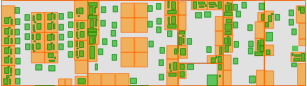
\includegraphics[width=\textwidth]{case-agh-rooms}
	\caption{Left-to-right, top-to-bottom: rooms 315, 316, 317, 317a, 318, and 319 of AGH UST C-3 building.}
	\label{fig:case-agh-rooms}
\end{figure}

\begin{itemize}
	\item two alternatives being quite different rooms 315 and 316 (\cref{lst:case-agh-315-316}),
	\item three seemingly similar rooms 317, 317a, and 318 (\cref{lst:case-agh-317-318}),
	\item and all rooms 315--319 (\cref{lst:case-agh-all}).
\end{itemize}

\begin{lstlisting}[label={lst:case-agh-315-316},caption={Mediation between rooms 315 and 316.}]
2 alternative(s) selected
JmlObject(../maps/C2-3rd-floor/Area.jml,room,POLYGON ((653 373, 653 366.5, 659.4 366.5, 659.4 373, 653 373)),Map(kind -> room, number -> 315))
JmlObject(../maps/C2-3rd-floor/Area.jml,room,POLYGON ((653 366.5, 653 359.7, 659.4 359.7, 659.4 366.5, 653 366.5)),Map(kind -> room, number -> 316))

Do you see some pc?
1: Yes
2: No
> 1
Possible alternatives left:
JmlObject(../maps/C2-3rd-floor/Area.jml,room,POLYGON ((653 366.5, 653 359.7, 659.4 359.7, 659.4 366.5, 653 366.5)),Map(kind -> room, number -> 316))

Chosen alternative: Some(JmlObject(../maps/C2-3rd-floor/Area.jml,room,POLYGON ((653 366.5, 653 359.7, 659.4 359.7, 659.4 366.5, 653 366.5)),Map(kind -> room, number -> 316))).
\end{lstlisting}

However similar, rooms 315 and 316 in \cref{lst:case-agh-315-316} have one major difference instantly visible in line 5. 316 contains lots of PCs, while 315 has none, being equipped with Apple iMacs. It is however possible that the user might have mistaken an iMac for a PC, ruining the correctness of the inference. In this case, the user answers ``Yes'' in line 8, and therefore room 316 is chosen (line 12).

\begin{lstlisting}[label={lst:case-agh-317-318},caption={Mediation between rooms 317, 317a, and 318.}]
3 alternative(s) selected
JmlObject(../maps/C2-3rd-floor/Area.jml,room,POLYGON ((654.67 359.7, 654.67 356.3, 659.4 356.3, 659.4 359.7, 654.67 359.7)),Map(kind -> room, number -> 317))
JmlObject(../maps/C2-3rd-floor/Area.jml,room,POLYGON ((653 359.7, 653 356.3, 654.67 356.3, 654.67 359.7, 653 359.7)),Map(kind -> room, number -> 317a))
JmlObject(../maps/C2-3rd-floor/Area.jml,room,POLYGON ((653 356.3, 653 353.2, 659.4 353.2, 659.4 356.3, 653 356.3)),Map(kind -> room, number -> 318))

Do you see some cupboard?
1: Yes
2: No
> 1
Possible alternatives left:
JmlObject(../maps/C2-3rd-floor/Area.jml,room,POLYGON ((653 356.3, 653 353.2, 659.4 353.2, 659.4 356.3, 653 356.3)),Map(kind -> room, number -> 318))

Chosen alternative: Some(JmlObject(../maps/C2-3rd-floor/Area.jml,room,POLYGON ((653 356.3, 653 353.2, 659.4 353.2, 659.4 356.3, 653 356.3)),Map(kind -> room, number -> 318))).
\end{lstlisting}

Here, in \cref{lst:case-agh-317-318}, because a cupboard is only present in room 318 (third alternative, line 4) and the user answers ``Yes'' (line 9), room 318 is chosen (line 13).

\begin{lstlisting}[label={lst:case-agh-all},caption={Mediation between all rooms 315--319.}]
6 alternative(s) selected
JmlObject(../maps/C2-3rd-floor/Area.jml,room,POLYGON ((653 353.2, 653 350.1, 659.4 350.1, 659.4 353.2, 653 353.2)),Map(kind -> room, number -> 319))
JmlObject(../maps/C2-3rd-floor/Area.jml,room,POLYGON ((654.67 359.7, 654.67 356.3, 659.4 356.3, 659.4 359.7, 654.67 359.7)),Map(kind -> room, number -> 317))
JmlObject(../maps/C2-3rd-floor/Area.jml,room,POLYGON ((653 356.3, 653 353.2, 659.4 353.2, 659.4 356.3, 653 356.3)),Map(kind -> room, number -> 318))
JmlObject(../maps/C2-3rd-floor/Area.jml,room,POLYGON ((653 373, 653 366.5, 659.4 366.5, 659.4 373, 653 373)),Map(kind -> room, number -> 315))
JmlObject(../maps/C2-3rd-floor/Area.jml,room,POLYGON ((653 366.5, 653 359.7, 659.4 359.7, 659.4 366.5, 653 366.5)),Map(kind -> room, number -> 316))
JmlObject(../maps/C2-3rd-floor/Area.jml,room,POLYGON ((653 359.7, 653 356.3, 654.67 356.3, 654.67 359.7, 653 359.7)),Map(kind -> room, number -> 317a))

Do you see some shelf unit?
1: Yes
2: No
> 2
Possible alternatives left:
JmlObject(../maps/C2-3rd-floor/Area.jml,room,POLYGON ((653 373, 653 366.5, 659.4 366.5, 659.4 373, 653 373)),Map(kind -> room, number -> 315))
JmlObject(../maps/C2-3rd-floor/Area.jml,room,POLYGON ((653 366.5, 653 359.7, 659.4 359.7, 659.4 366.5, 653 366.5)),Map(kind -> room, number -> 316))
JmlObject(../maps/C2-3rd-floor/Area.jml,room,POLYGON ((653 359.7, 653 356.3, 654.67 356.3, 654.67 359.7, 653 359.7)),Map(kind -> room, number -> 317a))

Do you see some fridge?
1: Yes
2: No
> 1
Possible alternatives left:
JmlObject(../maps/C2-3rd-floor/Area.jml,room,POLYGON ((653 359.7, 653 356.3, 654.67 356.3, 654.67 359.7, 653 359.7)),Map(kind -> room, number -> 317a))

Chosen alternative: Some(JmlObject(../maps/C2-3rd-floor/Area.jml,room,POLYGON ((653 359.7, 653 356.3, 654.67 356.3, 654.67 359.7, 653 359.7)),Map(kind -> room, number -> 317a))).
\end{lstlisting}

In the case of all six rooms (\cref{lst:case-agh-all}), two questions needed to be asked. In line 12, user said they saw no shelf unit, narrowing down possible alternatives' count to 3 (lines 13--16). Then, in line 21, they saw a fridge, resulting in room 317a being chosen as their position (line 25).

As claimed at the beginning of this chapter, there's no formal way for the algorithm to fail. Possible problems might arise from not naming the objects unambiguously enough or user making a mistake (in which case they can go back to a previous state of inference).

\section{Case 2: Main Square, Kraków}
\label{sec:case-cracow-square}

Although this paper is about \emph{indoor micro-location} via mediation, the mediation itself can also be used in other cases, e.g. outdoor location. This evaluation example---locating in sections of Main Square in Kraków---was explicitly asked for by the supervisor of this work.

\begin{figure}[b!]
	\centering
	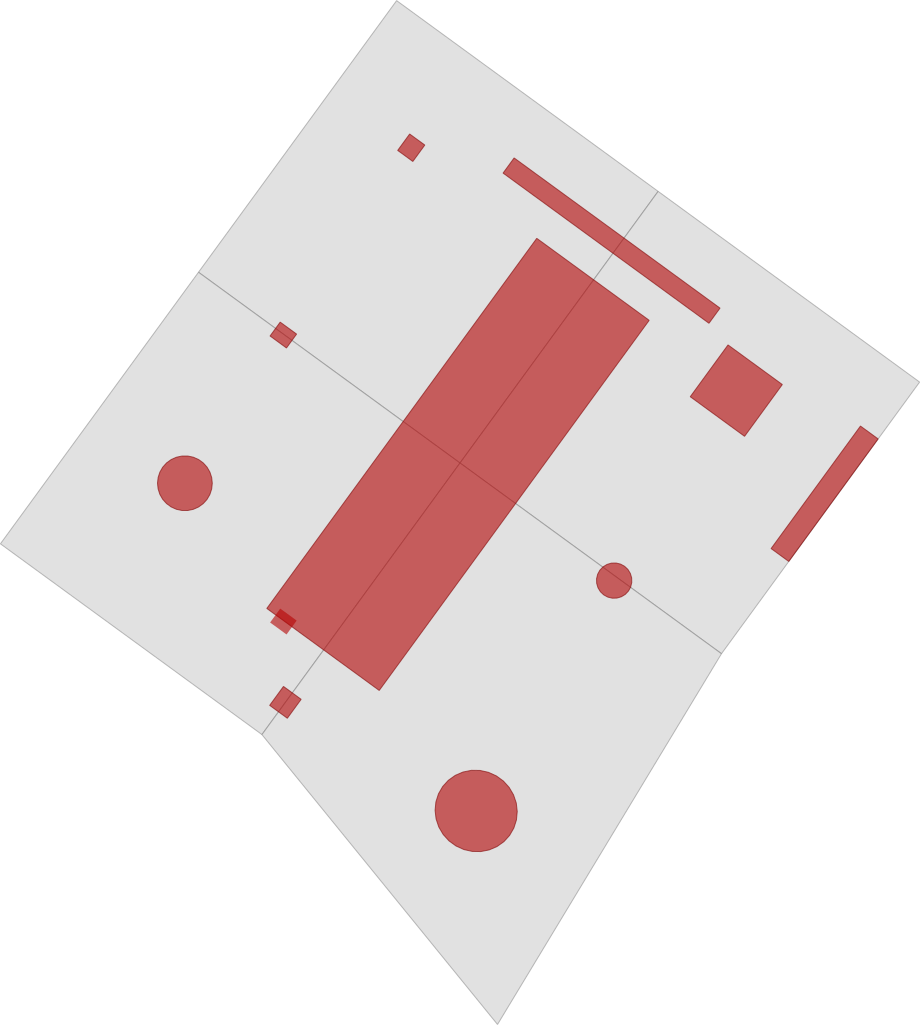
\includegraphics[width=0.67\textwidth]{case-cracow}
	\caption{The OpenGIS map used in the evaluated case of Main Square, Kraków.}
	\label{fig:case-cracow}
\end{figure}

\Cref{fig:case-cracow} represents simplified view of the Main Square in Kraków. It is divided into four gray quadrants: north, east, south, and west. These quadrants are the four discrete locations to which the user may be assigned in the process of mediation. The most distinctive ``features'' of the Main Square are marked on the maroon layer. These include: monuments, churches, Sukiennice, horse cab stand, etc.

Below, two sessions of mediation are shown.

\begin{lstlisting}[label={lst:case-cracow-one},caption={Mediation between all 4 quadrants. User is in the east one.}]
4 alternative(s) selected
JmlObject(../maps/Cracow-Main-Square/Area.jml,area,POLYGON ((538 277, 538 492, 745 492, 769 216, 538 277)),Map(quadrant -> South))
JmlObject(../maps/Cracow-Main-Square/Area.jml,area,POLYGON ((331 492, 331 707, 538 707, 538 492, 331 492)),Map(quadrant -> North))
JmlObject(../maps/Cracow-Main-Square/Area.jml,area,POLYGON ((331 277, 331 492, 538 492, 538 277, 331 277)),Map(quadrant -> West))
JmlObject(../maps/Cracow-Main-Square/Area.jml,area,POLYGON ((538 492, 538 707, 745 707, 745 492, 538 492)),Map(quadrant -> East))

Do you see Ratusz?
1: Yes
2: No
> 2
Possible alternatives left:
JmlObject(../maps/Cracow-Main-Square/Area.jml,area,POLYGON ((538 277, 538 492, 745 492, 769 216, 538 277)),Map(quadrant -> South))
JmlObject(../maps/Cracow-Main-Square/Area.jml,area,POLYGON ((331 492, 331 707, 538 707, 538 492, 331 492)),Map(quadrant -> North))
JmlObject(../maps/Cracow-Main-Square/Area.jml,area,POLYGON ((538 492, 538 707, 745 707, 745 492, 538 492)),Map(quadrant -> East))

Do you see studzienka Badylaka?
1: Yes
2: No
> 2
Possible alternatives left:
JmlObject(../maps/Cracow-Main-Square/Area.jml,area,POLYGON ((538 277, 538 492, 745 492, 769 216, 538 277)),Map(quadrant -> South))
JmlObject(../maps/Cracow-Main-Square/Area.jml,area,POLYGON ((538 492, 538 707, 745 707, 745 492, 538 492)),Map(quadrant -> East))

Do you see fontanna-piramida?
1: Yes
2: No
> 1
Possible alternatives left:
JmlObject(../maps/Cracow-Main-Square/Area.jml,area,POLYGON ((538 492, 538 707, 745 707, 745 492, 538 492)),Map(quadrant -> East))

Chosen alternative: Some(JmlObject(../maps/Cracow-Main-Square/Area.jml,area,POLYGON ((538 492, 538 707, 745 707, 745 492, 538 492)),Map(quadrant -> East))).
\end{lstlisting}

In \cref{lst:case-cracow-one}, in lines 11--14, after answering the first question, only 3 alternatives are left. Similarly, only 2 are left in lines 20--22. Finally, when the user is asked about ``fontanna-piramida,'' the only possible alternative left is the east quadrant (lines 29 and 31).

The obvious glaring problem here are the invisible walls between sections (quadrants) of the square. Arguably, during the first session, if the user was standing in the north quadrant, they would easily be able to see ``Ratusz,'' ``studzienka Badylaka,'' and ``fontanna-piramida.''

\begin{lstlisting}[label={lst:case-cracow-two},caption={Mediation between all 4 quadrants. User is in the north one.}]
4 alternative(s) selected
JmlObject(../maps/Cracow-Main-Square/Area.jml,area,POLYGON ((538 277, 538 492, 745 492, 769 216, 538 277)),Map(quadrant -> South))
JmlObject(../maps/Cracow-Main-Square/Area.jml,area,POLYGON ((331 492, 331 707, 538 707, 538 492, 331 492)),Map(quadrant -> North))
JmlObject(../maps/Cracow-Main-Square/Area.jml,area,POLYGON ((331 277, 331 492, 538 492, 538 277, 331 277)),Map(quadrant -> West))
JmlObject(../maps/Cracow-Main-Square/Area.jml,area,POLYGON ((538 492, 538 707, 745 707, 745 492, 538 492)),Map(quadrant -> East))

Do you see some ratusz?
1: Yes
2: No
> 1
Possible alternatives left:
JmlObject(../maps/Cracow-Main-Square/Area.jml,area,POLYGON ((331 277, 331 492, 538 492, 538 277, 331 277)),Map(quadrant -> West))

Chosen alternative: Some(JmlObject(../maps/Cracow-Main-Square/Area.jml,area,POLYGON ((331 277, 331 492, 538 492, 538 277, 331 277)),Map(quadrant -> West))).
\end{lstlisting}

\Cref{lst:case-cracow-two} is the illustration of that problem. The user is standing north, but---because they can see the ``Ratusz''---they answer ``yes'' in line 10. Their location is then incorrectly inferred to be the west quadrant.

The implementation works quite well for indoor spaces. However, currently, there's no concept of transparency (more on that in \cref{cha:summary}), resulting in mistakes in the second case.
